\section{Experiment}
\label{sec:experiment}

\shuqing{Experiment for devices and case study needed.}
For the purpose evaluating effectiveness of \tool, we conduct experiments in three modes on devices with USB Type-C interface.

Overview, \tool in experiments consist of a USB Type-C hub with HDMI and USB port,
a Raspberry Pi 4B with a Wi-Fi chip onboard,
a video capture card adapting HDMI signal to USB camera,
and a normal powerbank with dual outputs.
The powerbank is used to supply a piece of Raspberry Pi 4B and charge victim's device.
The USB Type-C hub adapts USB Type-C to a HDMI port and USB ports. The USB Type-C hub is used to connect HID devices and transmit video stream from victim's device to HDMI port. The video stream then will be capture by the Raspberry Pi 4B through the video capture card.

\subsection{Scripting mode}

In the scripting mode experiment, ``Lenovo Xiaoxin Pro 13 2020'', a PC in Windows 10 with two USB Type-C interfaces, is chosen as the target device. First, we connect \tool to the target device. Then \tool disguises itself as a normal keyboard. Like Rubber Ducky, \tool injects keystrokes at high speeds to perform using the hotkey to pull up a terminal (cmd.exe) and executing the malicious script in the terminal.

Through executing scripts, scripting mode can implant viruses, worms, backdoors, etc., which poses a significant risk to the victim's devices.
However, it can only be used on devices whose terminal is available, which limits its capability to PC.

\subsection{Remote control mode}

In the remote control mode experiment, ``iPad Pro (3rd generation)'', a tablet in iOS 14.3 with a USB Type-C interface, is chosen as the target device. First, we connect \tool to the target device.
Except performing as normal HID devices as Rubber Ducky, \tool can stream the real-time video output from the target device to the attacker through WiFi or GSM.
\tool capture video from USB Type-C Hub's HDMI output via a video capture card, stream video with ``FFmpeg'', a video processing utility and upload video stream to the attacker's device.
With a real-time video stream as an indicator, the attacker can precisely control the position of mouse movements and clicks. The attacker can control the iPad to open applications, peek at the victim's photos, etc.

Remote control mode is ideal for the attacker to control the victim's devices and grab all information shown on the victim's devices. However, it needs user consent for the first time and requires high power consumption to encode video streams and stable network connections.
In the real world, high power consumption will increase the posibilities of being noticed by the victim, and stable network connections is hardly guaranteed.


\subsection{Privacy extraction mode}

In the privacy extraction mode experiment, ``HUAWEI P30'', a smartphone in EMUI 9.1 (Android 9.0 based) with a USB Type-C interface, is chosen as the target device. 
First, we connect \tool to the target device. As remote control mode, \tool capture video from the victim's device and use ``opencv'' to identify ``valuable'' information from video stream. When the victim views text or photoes with text, \tool can use optical character recognition (OCR) to extract text from corresponding video frames. \yechang{hyperlink to OCR?}
For example, extracting the victim's name, photo, address, and ID number when victim is viewing his or her photos of his or her ID card or passport documents,
extracting the victim's payment information when victim is using bank apps or payment apps. Besides, \tool can use ``opencv'' to detect and decode QR codes or barcodes shown on the victim's device, which is expected to extract payment code information in payment apps.
Here is an example of extracting payment code with opencv library in listing. \shuqing{Need to be modified.}

Privacy extraction mode only extracts high-value information for attacker (or highly sensitive information for victim), which is more efficient to  than remote control mode.

%\begin{lstlisting}[caption={python script for extracting payment code of victim},label=lst2:qr]
%import cv2, qrcode,requests
%import pyzbar.pyzbar as pyzbar
%def decodeDisplay(video):
%    gray = cv2.cvtColor(video, cv2.COLOR_BGR2GRAY)
%    barcodes = pyzbar.decode(gray)
%    for barcode in barcodes:
%        barData = barcode.data.decode()
%        barType = barcode.type
%        requests.post('<server of attacker>',
%            data={
%                'data': barData,
%                'type': barType
%            }
%        )
%if __name__ == '__main__':
%    cam = cv2.VideoCapture(0)
%    while True:
%        ret, frame = cam.read()
%        decodeDisplay(frame)
%        if cv2.waitKey(5) == 27:
%            break
%    cam.release()
%    cv2.destroyAllWindows()
%\end{lstlisting}


\subsection{Case study}

We conduct a case study with Power bank sharing and QR code payment as technical background.

\subsubsection{Power bank sharing}

Power bank sharing provides users with short term rental of power banks. A provider deploys power bank stations in the city. Then, users can rent a power bank from any of the power bank station, charge their device on the trip, return the rented power bank to another station, and pay rent online.

As an example, Brick is such a power bank sharing service provider from Sweden. As Brick's website states, ``Brick prevents your electronics from running out of battery with powerbanks (Bricks) that you can easily rent \& return at our many stations in Stockholm, Gothenburg, Malmö and the rest of Sweden and even Europe.''. \yechang{citation needed}


\begin{figure}[hbtp]
	\centering
	\includegraphics[width=.4 \linewidth]{./Figs/Brick_station.png}
	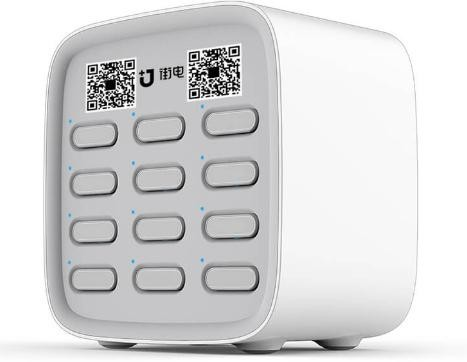
\includegraphics[width=.4 \linewidth]{./Figs/jiedian.jpg}
	\caption{Two power banks station products}\shuqing{Our attacking power banks.}
	\label{fig:PBS_products}
\end{figure}

\yechang{add hyperlink or reference to Brick's website or Brick App on App Store/Google Play.}

\yechang{Add more examples of power bank sharing to show that it is widely used?}

Whiling providing convenience for users, it brings security issues. We notice that the power bank station does not check the integrity of power banks during the rental process, and users are hardly cautious when connecting their devices to the power bank. A malicious user is able to modify his/her rented power bank, return it to a power bank station as normal, and its next user will unknowingly connect to this malicious power bank, which endangers the privacy of user.

\subsubsection{QR code payment}

QR code payment is a payment method where payment is typically performed as the following steps:
\ding{182} The payer opens the payment application on his/her mobile device, and present his/her payment QR code to the payee. This QR code is encoded with a globally unique ID to identify the payer's account. 
\ding{183} The payee scan the payment QR code presented by the payer. By presenting this QR code, the payer authorizes proceeding with the payment.
\ding{184} An order generated by this scan is sent to the payment service provider. Then the payment service provider requests the payer to confirm the transaction.
\ding{185} After confirmation, the payment service provider proceed with this transaction and return the payment result to both the payee and the payer.


\begin{figure}[hbtp]
	\centering
	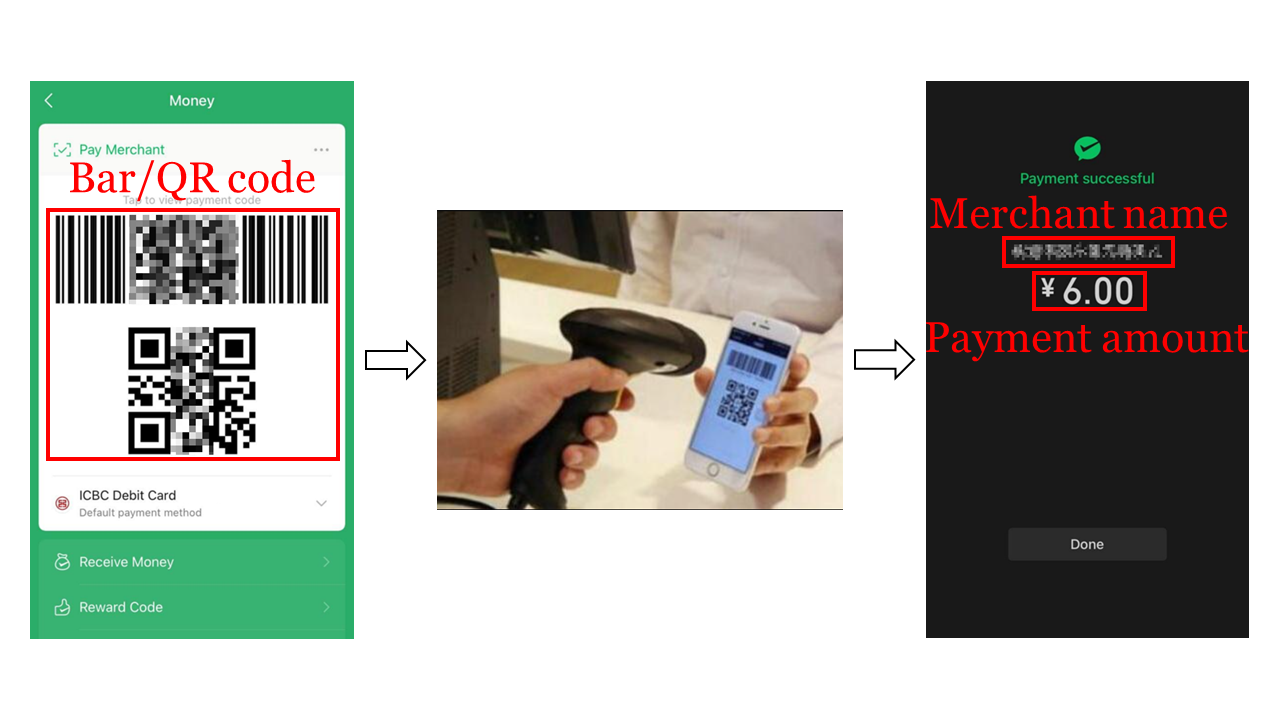
\includegraphics[width=\linewidth]{./Figs/qr_code_payment.png}
	\caption{Bar/QR code payment procedure}
	\label{fig:qr_payment_procedure}
\end{figure}


In the real-world, some payment service providers provide special rules for micropayments purchases. A micropayment is pre-determined by the payment service provider with thresholds in the user agreement. For example, WeChat Pay regards payments less than CNY \textyen 1000 as micropayments. Differing from a typical payment procedure, when micropayments are made, confirmations can be applied automatically without requiring the payer to take further action, which is often encouraged by the payment service provider.

The payment QR code is associated with the payer's account. If a victim's payment code is leaked to an attacker, an attacker can use the victim's payment code to proceed with payments. Furthermore, the attacker can use several micropayments to steal money from the victim's account while leaving the victim unconscious. In summary, the payment QR code is highly sensitive on users' devices.

\subsubsection{Attack scenario}

It is worth noting that \tool exposed only a type-c cable (from USB Type-C hub),
and \tool will charge his or her device through this cable, which has no difference from ordinary power banks. Noticed the low users' vigilance and high similarity between \tool and normal power bank, the attacker can return his/her modified power bank (as \tool) to a power bank station, mixing \tool into the circulation of shared power banks. The next user unconsciously connect his/her device to \tool. 
He/She can find his/her devices being charged as normal.
Like many outdoor mobile phone usage scenarios, the victim may complete payment with showing payment code. In this process, the attacker can preemptively extract and use the victim's payment code to make another payment unknown to the victim, which threatens victim's property.


\subsection{User study}

In order to check what can be obtained by \tool, we conduct a user study in order to check the performance of \tool in Privacy extraction mode.

\subsubsection{Setup}

\subsubsection{Scenario}

We invited 6 volunteers to our lab room. Volunteers take turns to operate their phones for half an hour while \tool is connected. Before the study, we did not reveal the function of \tool and asked the volunteers to connect their phones to \tool as a normal power bank (ignoring its larger size). 
After the study, we told them our attack, checked recorded videos together, and confirmed the consent to study the information in recorded videos, Subject to efficiency reasons, we ask them to use phones like when they use the shared power bank outside.


\subsubsection{Result}

After collecting the videos, we used both automatic and manual methods to analyze the video. In the automatic analysis, we use a script to simply perform OCR recognition to each frame in the recorded video and store all OCR results into a database in a format of ``frame number - text by OCR''. At last, there are 38329 pieces of data collected among 6 volunteers. In the manual analysis, we replay the recorded video and extract sensitive information manually.

In terms of automatic analysis, OCR results of all frames are already stored in the database and can be used at hand. With these results, we can learn what issues the victim is browsing. Additionally, some keywords often appear with users' input data because they are often used as labels of input boxes, such as ``account'', ``username''. Such keywords are more likely to lead us to discover user-specific data. For example, in Figure~\ref{fig:ocr_keyword_example}, searching with ``account'' as the keyword, victim's accounts can be detected as shown in Fig. The frame number is the position of this frame in the recorded video, which indicates a target for manual analysis for further data extraction.

\begin{figure}[hbtp]
	\centering
	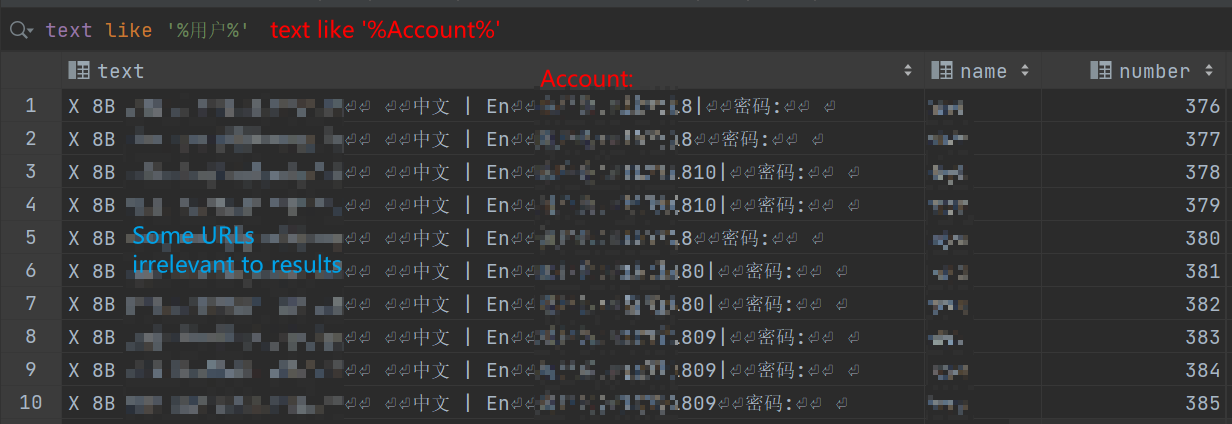
\includegraphics[width=\linewidth]{./Figs/ocr_keyword_example.png}
	\caption{Search ``account'' in all OCR results}
	\label{fig:ocr_keyword_example}
\end{figure}

In terms of manual analysis, data collected are listed in table ~\ref{table:information_extracted}. Accounts of internet applications such as Apple ID, iCloud, Facebook, Twitter, WeChat, QQ, Alipay can be obtained. Additionally, all typing inputs are on the virtual keyboard (including the system keyboard and the built-in security keyboard of the financial app), which can be clearly recorded. Noticed that, we can obtain the plain text of password typed such as the WiFi password and the Alipay password. Furthermore, the received SMS verification code (usually is used to confirm real-name authentication) can be obtained when it appears in the top notification bar. 


In summary, we can no longer directly peek at the user’s password on the lock screen. But if the user unconsciously unlocks the screen, we can still check all information presented on the screen, extract private information including but not limited to social accounts, bank accounts, personal financial situation, etc. It is worth noting that the so-called secure keyboards built into some financial apps just simply disrupt the keyboard sequence and cannot prevent attacks similar to \tool.


\begin{table*}[hbtp]
	\centering
	\begin{tabular}{|c|c|c|c|c|}
		\hline
		Application Column  & Application & Private information leaked                       \\
		\hline
		Finance App         & Alipay      & Alipay account, personal assets(blance)          \\
		\hline
		Social  Finance App & WeChat      & WeChat account, blance, chat history             \\
		\hline
		Social App          & QQ          & QQ account, interpersonal nexus, chat history    \\
		\hline
		Social App          & Twitter     & Twitter account, interpersonal nexus             \\
		\hline
		Social App          & Gmail       & Gmail account, mail records                      \\
		\hline
		Finance App         & ICBC        & ICBC account, password, personal assets(blance)  \\
		\hline
		Finance App         & Paypal      & Paypal account, blance, bank accounts            \\
		\hline
		Tool                & Chrome      & Sites visited                                    \\
		\hline
		Tool                & Health      & personal physical metrics      					 \\
		\hline
	\end{tabular}
	\linebreak
	\caption{Information extracted}
	\label{table:information_extracted}
\end{table*}